\chapter{系统实现与实验结果}
\label{chap04}

\section{原型系统设计与实现}
为了便于展示实验结果,本文设计并实现了一个原型系统,称作SMap。
系统采用浏览器/服务器(Browser/Server)架构,在服务器端进行计算,计算完成后通过
web页面呈现结果。服务器端采用Java Servlet实现,浏览器端采用AJAX技术,可以完成异
步请求,即在不刷新整个页面的情况下完成和服务器之间的通信以及部分页面的更新。

服务器端架构如图\ref{fig:server}所示,根据不同模块的功能可分为三个部分:解析部分
、简单映射发现部分以及复杂映射发现部分。

\begin{figure}[htbp]
\centerline{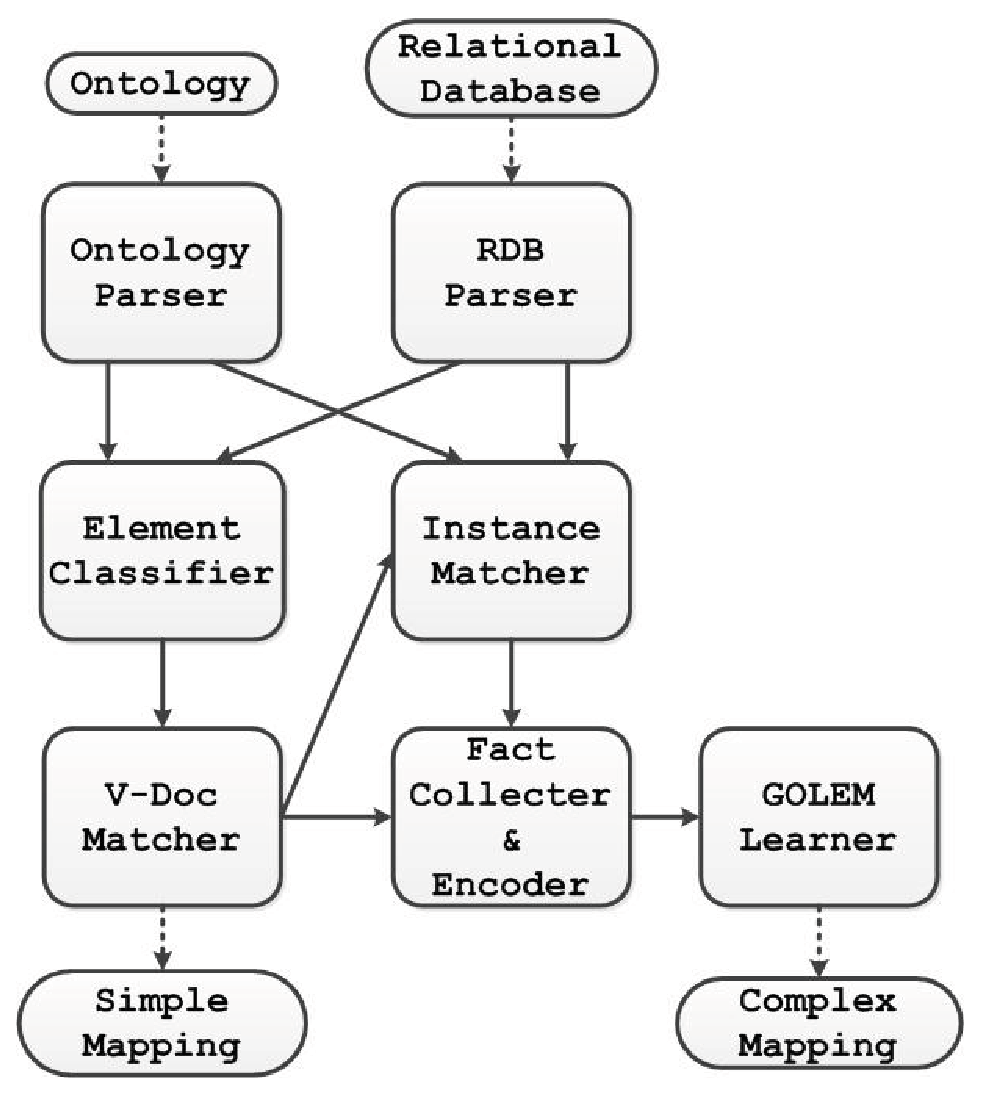
\includegraphics[height=10cm]{server}}
\caption{服务器端架构}
\label{fig:server}
\end{figure}

解析部分包含两个解析器:关系数据库解析器以及本体解析器。关系数据库解析器将用户
输入的关系数据库URL解析为关系数据库模式的元素(如表和列)及其实例(元组);本体
解析器用于将用户输入的本体URL解析为本体元素(如类和属性)及其实例(RDF数据),
解析时采用了开源的Jena API\footnote{\url{http://jena.apache.org}}。

简单映射部分包含元素分类器以及虚拟文档匹配器。元素分类器接收解析出的元素,然后
根据\ref{2:1}节中提到的分类规则将关系数据库模式和本体中的元素划分为不同的类别,
再将分类后的元素输入虚拟文档匹配器;虚拟文档匹配器在接收到不同类别的关系数据库
模式和本体元素后,采用\ref{2:2}节中的方法,对每个元素建立虚拟文档,然后计算元素
间的相似度,选取简单映射。

复杂映射部分包含实例匹配器、事实收集编码器以及GOLEM学习器。实例匹配器除了接收经
过解析的关系数据库和本体实例数据之外,还需要以已经发现的简单映射作为依据进行实例
数据的匹配;实例匹配器将经过匹配的重叠实例数据输入事实收集编码器中,事实的收集同
样需要将已经发现的简单映射作为依据,在收集到事实之后需要将其编码为谓词逻辑形式,
输入GOLEM学习器;GOLEM学习器根据输入的背景知识和正例进行学习,最终得到Horn规则
表示的复杂映射。

浏览器端界面如图\ref{fig:interface}所示,可通过web浏览器进行访问
\footnote{\url{http://ws.nju.edu.cn/smap}}。
用户可在该页面输入关系数据库模式和本体的URL以及需要发现的语义映射类型,系统完成
语义映射的发现后可将结果即时呈现在页面上。

\begin{figure}[htbp]
\centerline{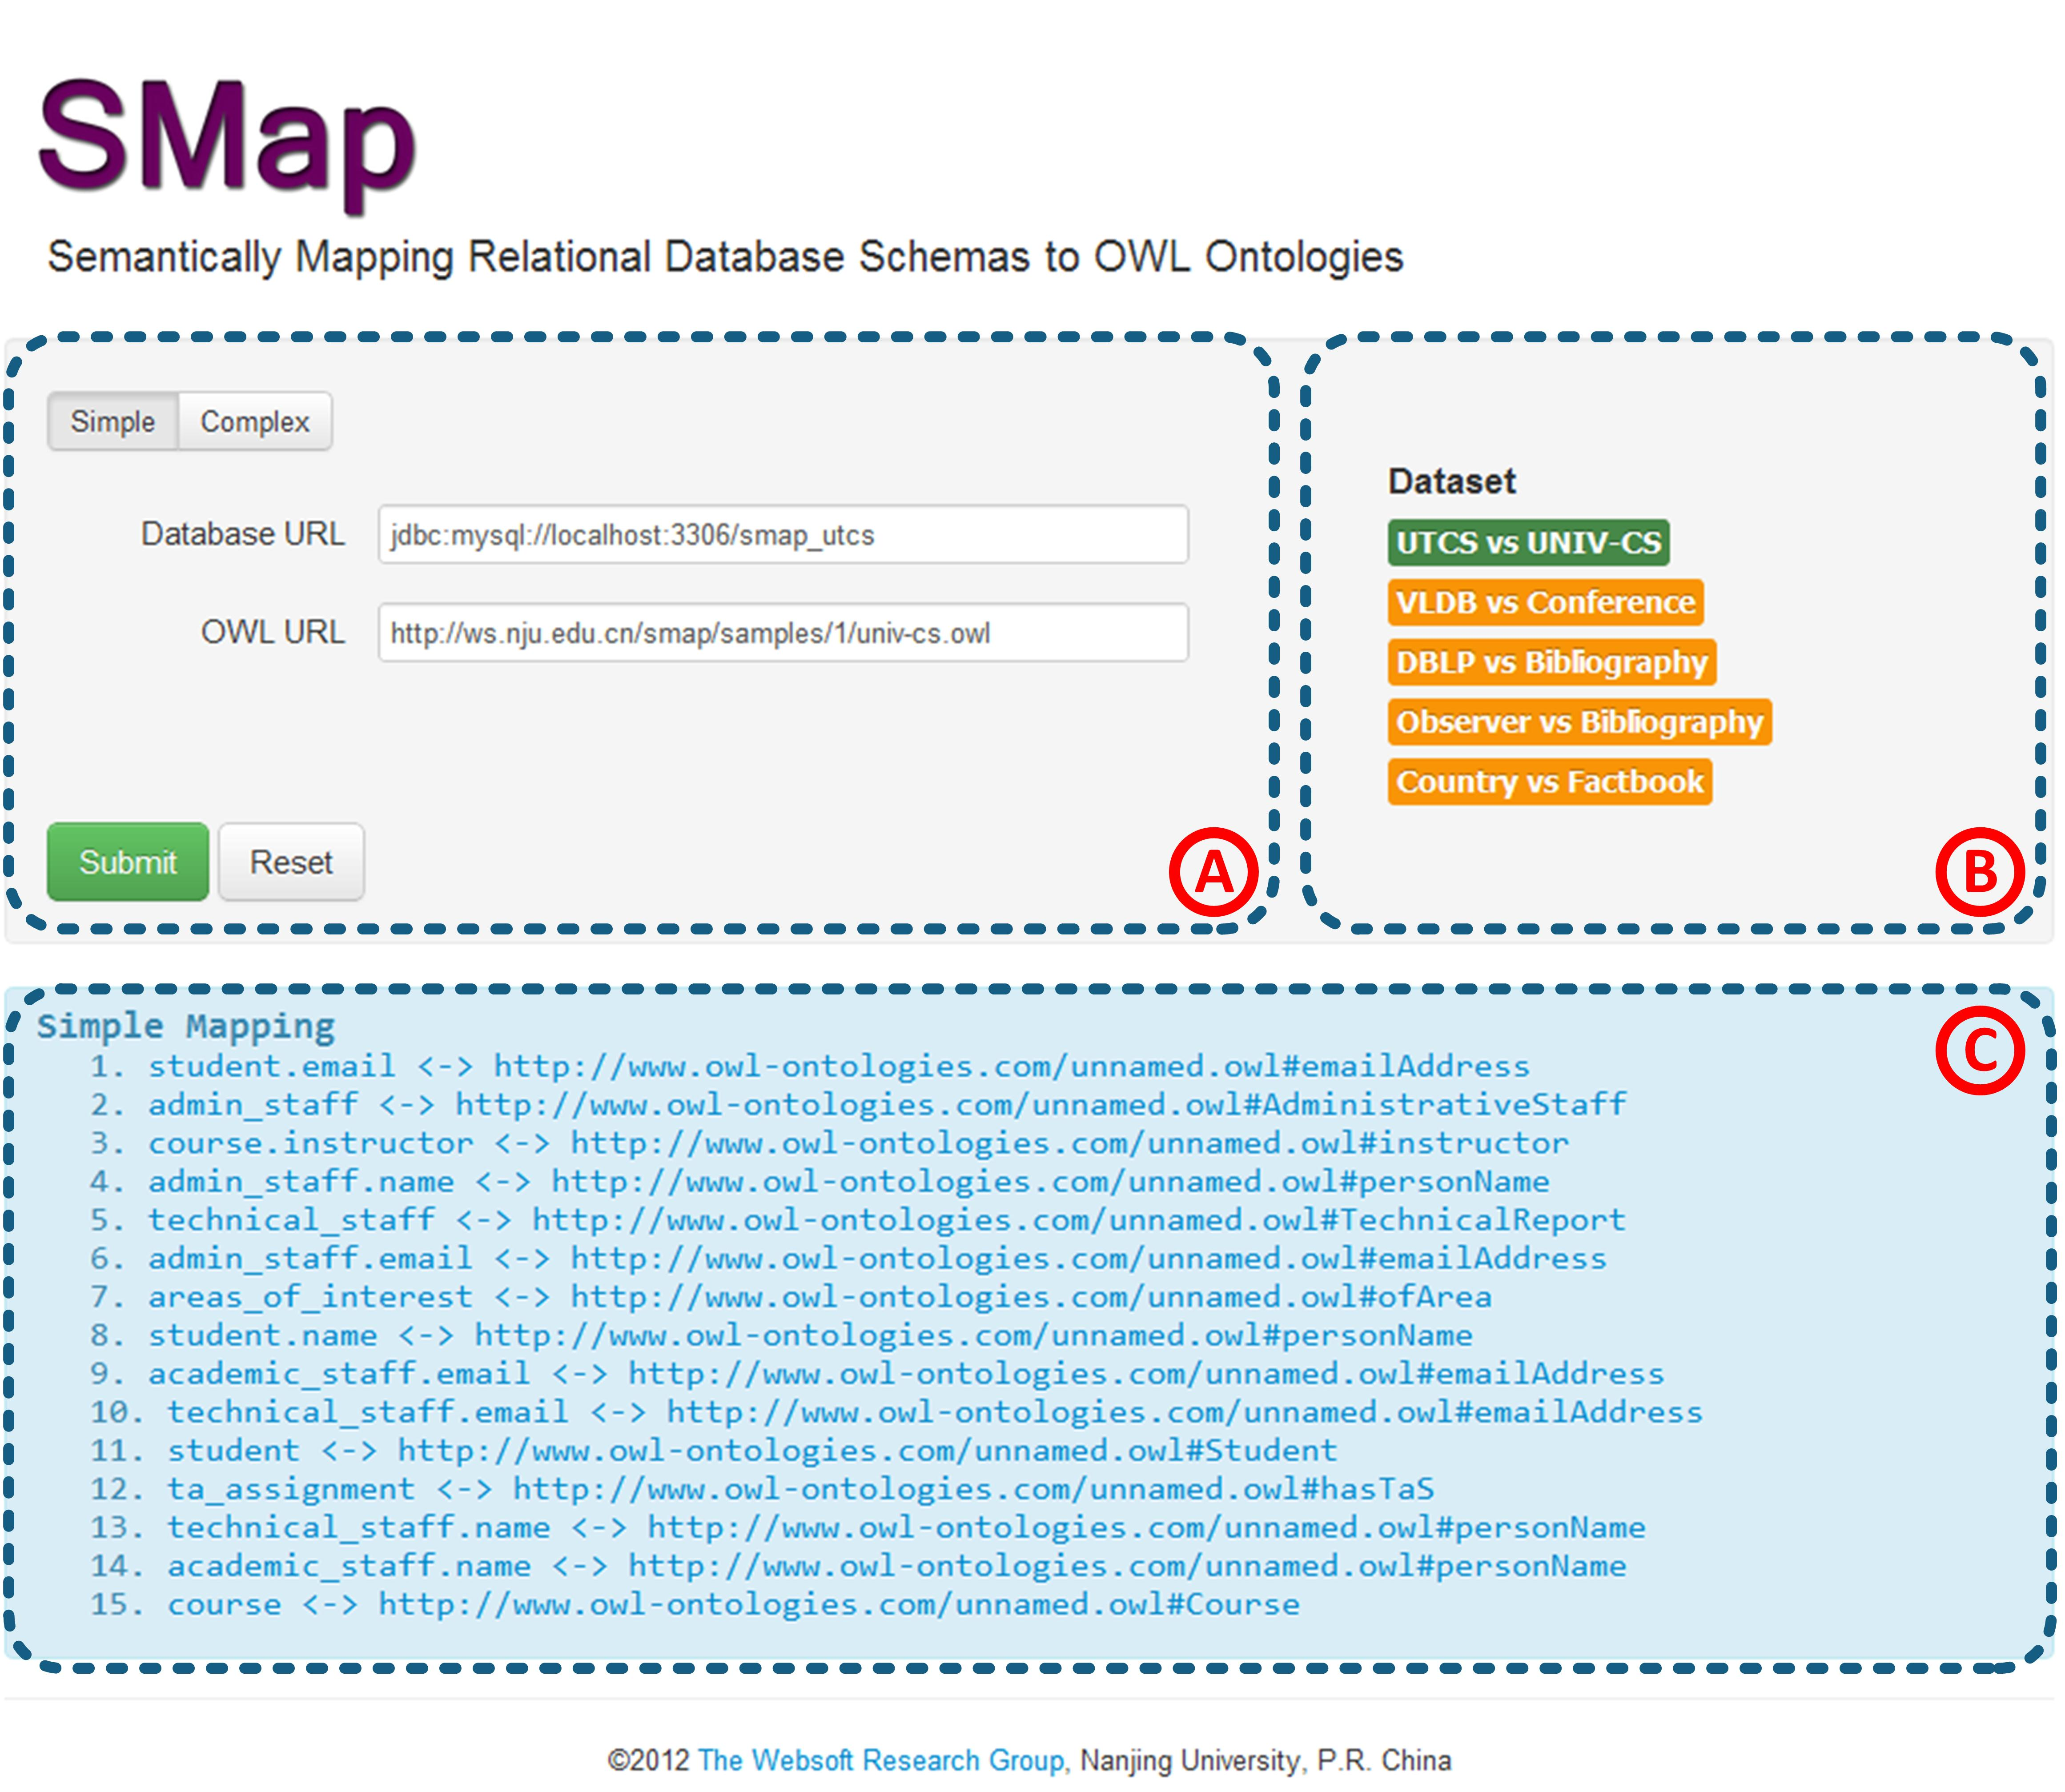
\includegraphics[width=10cm]{interface}}
\caption{浏览器端界面}
\label{fig:interface}
\end{figure}

界面主要分为3个区域,区域A为输入区,左上角的按钮用于选择需要进行发现的语义映射
类型为简单或是复杂,按钮下方的表单用于接收数据集的URL,表单下方的按钮用于提交
或重置;区域B为示例数据集区,通过点击数据集条目可将对应的示例数据集的URL自动填
入输入区中;区域C为结果区,用于呈现系统发现的语义映射。

\section{实验结果与分析}

实验选用6组测试数据集,表\ref{tab1}列出了这些测试集的统计信息。其中,前5组测试
集由MapOnto\cite{10}发布,而IBM WCC测试集由IBM公司提供。这些测试集来源于真实世
界的不同领域,并且每个测试集中的关系数据库模式与本体均相互独立。

\begin{table}[htbp]
\centering
\caption{测试数据集}
\label{tab1}
\begin{tabular}{lrrlrrrr}
\hline
\multirow{2}{*}{数据库} & \multirow{2}{*}{\#表}&\multirow{2}{*}{\#列}&
\multirow{2}{*}{本体}&\multirow{2}{*}{\#类}&\multirow{2}{*}{\#属性} &
\multicolumn{2}{c}{\#参考映射}\\
\cline{7-8}
&&&&&&简单&复杂\\
\hline
UTCS		&8	&32	&Univ-CS	&53	&35	&18	&6\\
VLDB		&9	&38	&Conference	&18	&29	&27	&4\\
DBLP		&5	&27	&Bibliography	&66	&81	&21	&4\\
Observer	&8	&115	&Bibliography	&66	&81	&72	&6\\
Country		&6	&18	&Factbook	&43	&209	&22	&5\\
IBM WCC		&279	&2187	&New WCC	&79	&276	&274	&\\
\hline
\end{tabular}
\end{table}

下面分别在简单映射发现和复杂映射学习这两个方面开展实验,并与现有工具方法进行对比
。使用精度、召回率以及F-Measure
\footnote{$\textit{F-Measure} =
\frac{2 \times \textit{召回率} \times \textit{精度}}
{\textit{召回率} + \textit{精度}}$}
(精度和召回率的线性组合)评价实验结果。评价过程中使用的参考映射由5名受过训练
的研究生手工创建。实验环境为一台拥有4GB内存的普通PC机。

\subsection{简单映射发现的实验结果与分析}
在简单映射发现方面,设计了3个对比实验来测试SMap的性能。

\theoremstyle{definition}
\newtheorem{experiment}{\heiti{实验}}
\begin{experiment}
关系数据库模式和本体中的元素是否分类对SMap的影响。这里仅使用元素自身的自然语言
描述来计算元素之间的相似度。
\end{experiment}

\begin{experiment}
\label{exp2}
是否引入相邻元素的自然语言描述对于SMap的影响,以及何种相邻元素的对结果的影响最
大。本实验中对元素进行了类型分类。相关参数设置如下:
$\alpha=0.2 \mbox{、}\beta=0.1$。在这组参数下,SMap也取得了最好的平均F-Measure。
\end{experiment}

\begin{experiment}
对比SMap与其它3个映射工具的性能。COMA++\cite{21}是目前功能最完备的映射工具之一,
它将输入模型统一转换为有向无环图的结构,因此能发现关系数据库模式与本体间的映射。
COMA++包含多种映射算法并设置了不同的映射结果组合策略。Lily\cite{22}和
AROMA\cite{23}是两个本体映射工具。本实验中先使用D2RQ将关系数据库模式转化为本体,
再分别使用它们实施本体与本体之间的映射。
\end{experiment}

图\ref{fig2}展示了是否考虑元素类型分类的对比结果。从图中可以看出,在所有测试集
中,考虑元素分类的F-Mearsure要一致优于不考虑元素分类的结果。
\begin{figure}[htbp]
\centerline{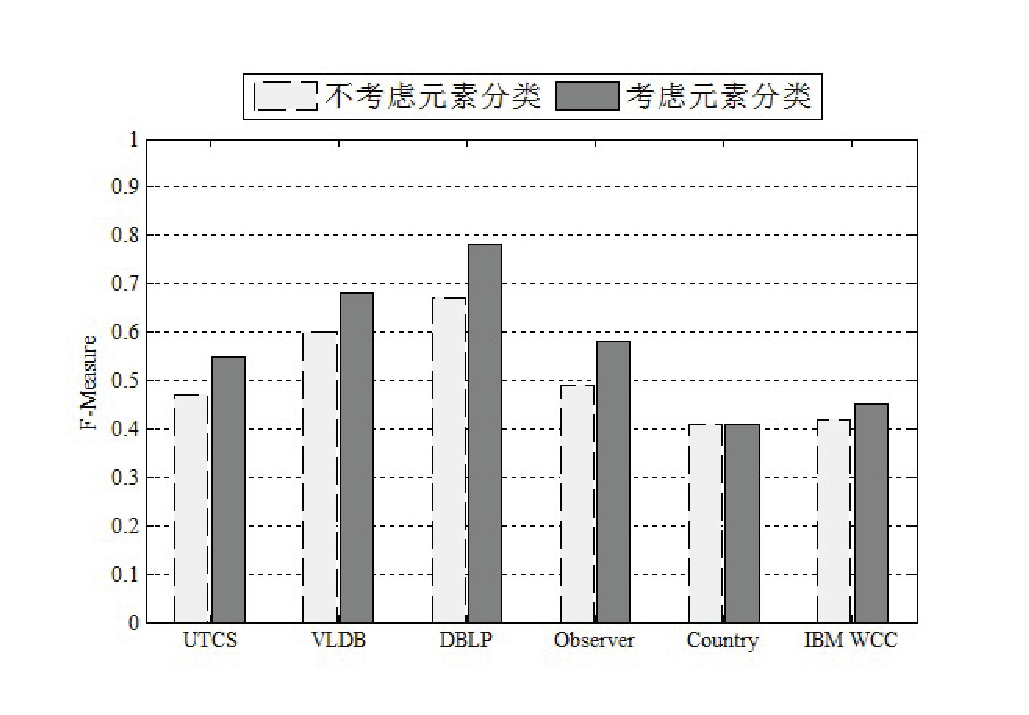
\includegraphics[width=8cm]{2}}
\caption{不考虑元素类型分类与考虑元素类型分类的F-Measure对比}
\label{fig2}
\end{figure}

实验\ref{exp2}的对比结果在图\ref{fig3}中给出。考虑相邻元素能够显著提高SMap的
F-Measure。原因在于大部分测试集中元素自身的自然语言描述较少,使用相邻元素的
描述有助于发现更多的简单映射。

\begin{figure}[htbp]
\centerline{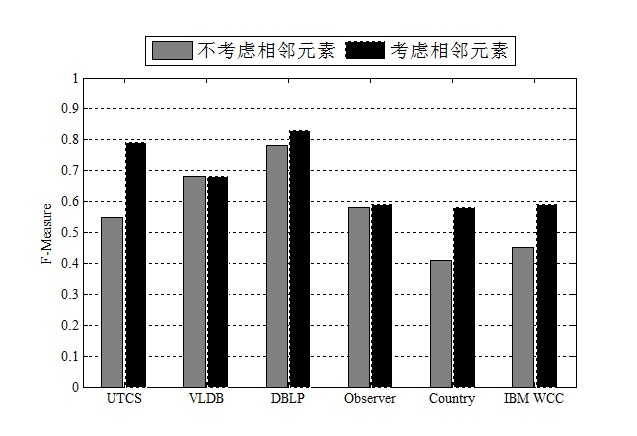
\includegraphics[width=8cm]{3}}
\caption{不考虑相邻元素和考虑相邻元素的F-Measure对比}
\label{fig3}
\end{figure}

另外,实验还对相邻元素进行了细分,发现引入关系数据库和本体属性的定义域元素对
效果提升明显,而考虑属性值域的数据类型有时反而会起到副作用,这是由于许多不同
属性都拥有相同的数据类型例如(字符型),干扰了相似度的计算。

图\ref{fig4}展示了SMap与其他3种方法在6组测试集下的平均值。精度上,SMap优于
COMA++和Lily,比AROMA差。而召回率上,SMap要明显优于其它所有工具。每个测试集的
F-Measure可参见汇总表\ref{tab2}的简单映射部分。从该表可以看出,SMap的平均
F-Measure超过其他工具20\%以上。


\begin{figure}[htbp]
\centerline{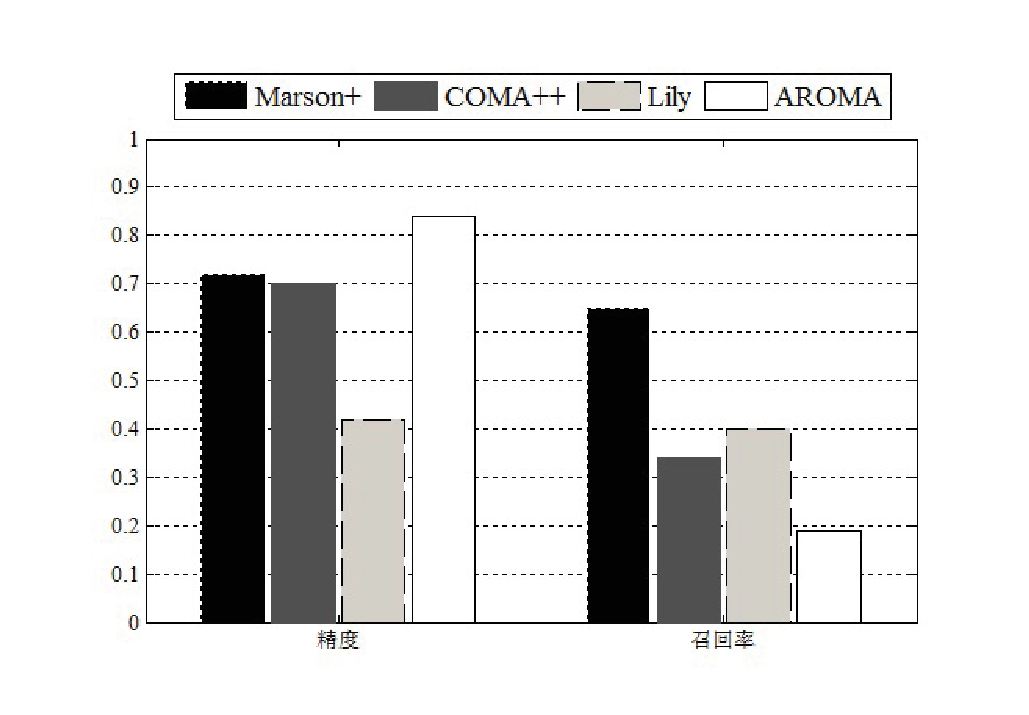
\includegraphics[width=8cm]{4}}
\caption{简单映射发现的平均精度和召回率对比}
\label{fig4}
\end{figure}


\subsection{复杂映射学习的实验结果与分析}
\begin{experiment}
比较SMap、MapOnto\cite{10}和Marson\cite{24}学习到的复杂语义映射的精度和召回率。
MapOnto需要预先构建的简单映射作为复杂映射的学习输入,故将SMap发现的简单映射输入
MapOnto。另外由于IBM WCC测试集没有公开的实例数据,因此无法在此实验中使用。
\end{experiment}

\begin{table}[htbp]
\centering
\caption{各种方法的详细实验结果汇总}
\label{tab2}
\footnotesize
\begin{tabular}{ccccccccc}
\hline
\multicolumn{2}{l}{度量指标:F-Measure} &UTCS &VLDB &DBLP &Observer &Country
&IBM WCC &平均值\\
\hline
简单映射&SMap&0.79&0.68&0.83&0.59&0.58&0.59&0.68\\
	&COMA++&解析报错&0.45&0.57&0.38&0.47&0.41&0.46\\
	&Lily&0.50&0.47&0.43&0.44&0.37&0.21&0.40\\
	&AROMA&0.29&0.43&0.25&0.10&0.43&0.32&0.30\\
\hline
复杂映射&SMap&0.92&0.89&0.86&0.67&0.73&&0.81\\
	&MapOnto&0.50&0.67&0.67&0.50&0.75&&0.62\\
	&Marson&0.50&0.40&0.40&&&&0.43\\
\hline  
\end{tabular}
\end{table}

从图\ref{fig5}的结果能够看出,3种工具的平均精度都很高,Marson更是达到了1.0。
而SMap的精度会收到实例匹配的影响。从召回率来看,SMap比其他2种工具明显要好。
通过观察其他2种工具找到的复杂映射可以发现,MapOnto主要发现了类型\ref{typ1}
的复杂映射,而Marson主要发现了类型\ref{typ3}的复杂映射。在实际数据集中,属于类
型\ref{typ1}的复杂映射最多,类型\ref{typ2}次之,类型\ref{typ3}最少,这也造成了
Marson的召回率要低于MapOnto。在运行时间方面,由于MapOnto不需要实例数据,故执行
速度较快,完成每个数据集平均耗时约0.5s。而在有200个重叠实例数据的情况下,
Marson在每个数据集上的学习耗时约1s,SMap需要约2s(仅在复杂映射学习阶段)。
\begin{figure}[htbp]
\centerline{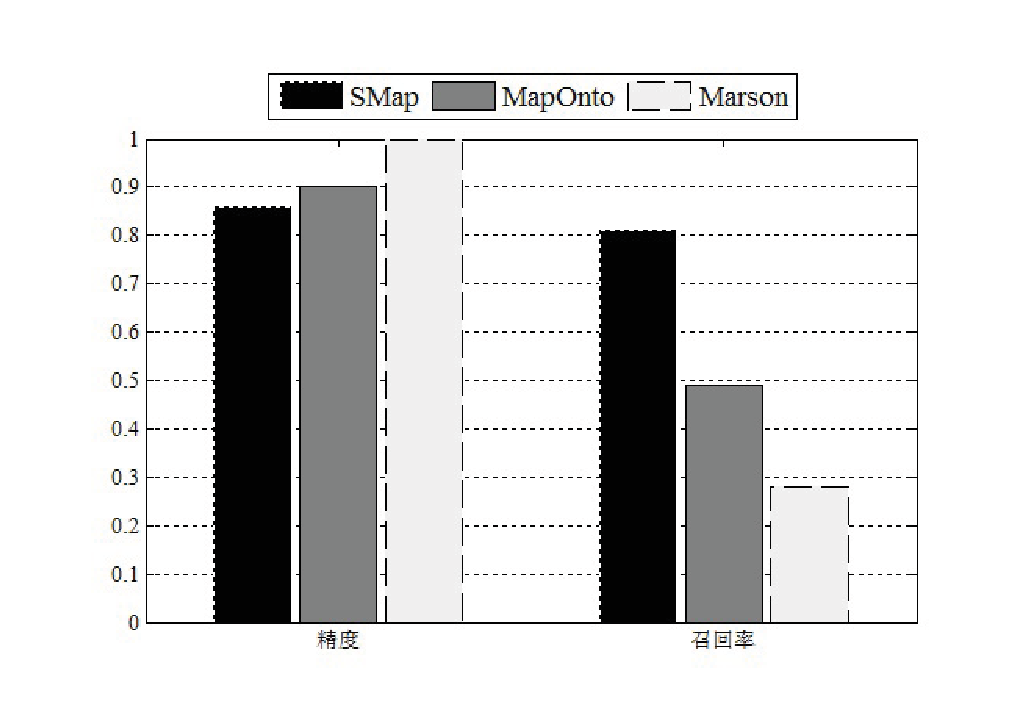
\includegraphics[width=8cm]{5}}
\caption{复杂映射学习的平均精度和召回率对比}
\label{fig5}
\end{figure}


以下为SMap学习到的一部分复杂映射:
\begin{itemize}
\item{
\textbf{\emph{DBLP}}:\emph{publisher}(\emph{name,addr}) :-
\textbf{\emph{Bibliography}}:\emph{Publisher}(\emph{A}),
\flushright{
\textbf{\emph{Bibliography}}:\emph{Agent\_name}(\emph{A,name}),
\textbf{\emph{Bibliography}}:\emph{Publisher\_Address}(\emph{A,addr}).
}}
\item{
\textbf{\emph{UTCS}}:\emph{ta\_assignment}(\emph{ctitle,sname}) :-
\textbf{\emph{Univ-CS}}:\emph{hasTaS}(\emph{B,A}),
\flushright{
\textbf{\emph{Univ-CS}}:\emph{GraduateStudent}(\emph{A}),
\textbf{\emph{Univ-CS}}:\emph{personName}(\emph{A,sname}),
\textbf{\emph{Univ-CS}}:\emph{Course}(\emph{B}),
\textbf{\emph{Univ-CS}}:\emph{courseTitle}(\emph{B,ctitle}).
}}
\item{
\textbf{\emph{VLDB}}:\emph{event}(\emph{title,\_,type,\_,\_,\_,\_}) :-
\textbf{\emph{Conference}}:\emph{Presentation}(\emph{A}),
\flushright{
\textbf{\emph{Conference}}:\emph{eventTitle}(\emph{A,title}).
}}
\end{itemize}


